\documentclass[aspectratio=169]{beamer}

\mode<presentation>
{
  \usetheme{default}
  \usecolortheme{default}
  \usefonttheme{default}
  \setbeamertemplate{navigation symbols}{}
  \setbeamertemplate{caption}[numbered]
  \setbeamertemplate{footline}[frame number]  % or "page number"
  \setbeamercolor{frametitle}{fg=white}
  \setbeamercolor{footline}{fg=black}
} 

\usepackage[english]{babel}
\usepackage[utf8x]{inputenc}
\usepackage{tikz}
\usepackage{courier}
\usepackage{array}
\usepackage{bold-extra}
\usepackage{minted}
\usepackage[thicklines]{cancel}

\xdefinecolor{dianablue}{rgb}{0.18,0.24,0.31}
\xdefinecolor{darkblue}{rgb}{0.1,0.1,0.7}
\xdefinecolor{darkgreen}{rgb}{0,0.5,0}
\xdefinecolor{darkgrey}{rgb}{0.35,0.35,0.35}
\xdefinecolor{darkorange}{rgb}{0.8,0.5,0}
\xdefinecolor{darkred}{rgb}{0.7,0,0}
\definecolor{darkgreen}{rgb}{0,0.6,0}
\definecolor{mauve}{rgb}{0.58,0,0.82}

\title[2018-02-16-gpu-programming]{First steps in GPU programming}
\author{Jim Pivarski}
\institute{Princeton University -- DIANA-HEP}
\date{February 16, 2018}

\begin{document}

\logo{\pgfputat{\pgfxy(0.11, 7.4)}{\pgfbox[right,base]{\tikz{\filldraw[fill=dianablue, draw=none] (0 cm, 0 cm) rectangle (50 cm, 1 cm);}\mbox{\hspace{-8 cm}
\includegraphics[height=1 cm]{princeton-logo-long.png}
\includegraphics[height=1 cm]{diana-hep-logo-long.png}}}}}

\begin{frame}
  \titlepage
\end{frame}

\logo{\pgfputat{\pgfxy(0.11, 7.4)}{\pgfbox[right,base]{\tikz{\filldraw[fill=dianablue, draw=none] (0 cm, 0 cm) rectangle (50 cm, 1 cm);}\mbox{\hspace{-8 cm}
\includegraphics[height=1 cm]{princeton-logo.png}
\includegraphics[height=1 cm]{diana-hep-logo.png}}}}}

% Uncomment these lines for an automatically generated outline.
%\begin{frame}{Outline}
%  \tableofcontents
%\end{frame}

% START START START START START START START START START START START START START

\begin{frame}{Goal: running your own algorithms on the GPU}
\vspace{0.5 cm}
\large
This talk is not about high-level machine learning tools that {\it use} the GPU, but directly programming it for physics.

\begin{enumerate}
\item How to install the software.
\item Three ways to write code: (1) nvcc, (2) PyCUDA, (3) Numba.
\item What to consider: good GPU algorithms and bad GPU algorithms.
\item How to get the data (uproot, of course).
\end{enumerate}
\end{frame}

%% \begin{frame}[fragile]{Getting started}
%% \vspace{0.5 cm}
%% \large

%% {\bf Step 1:} get a GPU (legally).

%% \vspace{0.25 cm}
%% {\bf Step 2:} install CUDA: \textcolor{blue}{\normalsize \underline{\url{https://developer.nvidia.com/cuda-downloads}}}

%% \vspace{0.5 cm}
%% On Ubuntu, it looked like
%% \small
%% \begin{minted}{bash}
%% wget "https://developer.nvidia.com/compute/cuda/8.0/Prod2/local_"\
%% "installers/cuda-repo-ubuntu1604-8-0-local-ga2_8.0.61-1_amd64-deb"
%% sudo dpkg -i cuda-repo-ubuntu1604-8-0-local-ga2_8.0.61-1_amd64-deb  
%% sudo apt-get update
%% sudo apt-get install cuda
%% \end{minted}

%% \large
%% \vspace{0.5 cm}
%% {\bf Alternatively:} log into {\tt cmslpcgpu1.fnal.gov} (or {\tt 2} or {\tt 3}).

%% \small
%% \begin{minted}{bash}
%% export CUDA_HOME=/usr/local/cuda
%% export LD_LIBRARY_PATH=$CUDA_HOME/lib64:$LD_LIBRARY_PATH
%% export PATH=$CUDA_HOME/bin:$PATH
%% \end{minted}
%% \end{frame}

%% \begin{frame}[fragile]{Now you can write GPU programs with nvcc}
%% \vspace{0.25 cm}
%% \scriptsize
%% \begin{minted}{c++}
%% #include <cstdlib>
%% #include <iostream>
%% const int MILLION = 1024*1024; float cpu_datain[MILLION]; float cpu_dataout[MILLION];

%% __global__ void gpu_kernel(float* datain, float* dataout) {
%%   int id = threadIdx.x + blockIdx.x*blockDim.x;
%%   dataout[id] = sqrt(datain[id]);
%% }

%% int main(int argc, char**argv) {
%%   srand(12345);
%%   for (int i = 0;  i < MILLION;  i++) cpu_datain[i] = ((float)rand()) / RAND_MAX;

%%   float* gpu_datain; float* gpu_dataout;
%%   cudaMalloc((void**)&gpu_datain, MILLION*sizeof(float));
%%   cudaMalloc((void**)&gpu_dataout, MILLION*sizeof(float));
%%   cudaMemcpy(gpu_datain, cpu_datain, MILLION*sizeof(float), cudaMemcpyHostToDevice);
%%   gpu_kernel<<<MILLION / 1024, 1024>>>(gpu_datain, gpu_dataout);
%%   cudaMemcpy(cpu_dataout, gpu_dataout, MILLION*sizeof(float), cudaMemcpyDeviceToHost);

%%   std::cout << "first: " << cpu_datain[0] << " --> " << cpu_dataout[0] << std::endl;
%%   return 0;
%% }
%% \end{minted}
%% \end{frame}

%% \begin{frame}[fragile]{What did we just do?}
%% \vspace{0.5 cm}
%% \begin{enumerate}
%% \item The GPU has an entirely different machine code than the CPU, and nvcc compiles some parts of the program for CPU, some for GPU.
%% \item Functions defined with {\small\tt \_\_global\_\_} are compiled to run on GPU, called by CPU.
%% \item Thousands of {\small\tt gpu\_kernel} functions run at once. Each determines its part of the problem from its {\small\tt id = threadIdx.x + blockIdx.x*blockDim.x}.
%% \item Some pointers point at memory on GPU (segfault to access them from CPU).
%% \item Data must be explicitly copied from CPU arrays to GPU arrays (and back).
%% \item Calling a GPU function, you have to specify ``number of blocks'' and \mbox{``block size'':\hspace{-0.5 cm}}
%% \small
%% \vspace{0.25 cm}
%% \begin{minted}{c++}
%% gpu_kernel<<<numblocks, blocksize>>>(gpu_datain, gpu_dataout);
%% \end{minted}

%% \vspace{0.25 cm}
%% \normalsize
%% The {\small\tt blocksize} is number to run at once (usually max is 1024) and {\small\tt numblocks} is the number of such blocks.
%% \end{enumerate}
%% \end{frame}

%% \begin{frame}{What are blocks?}
%% \vspace{0.5 cm}

%% \Large
%% Tuning parameter for the {\it algorithm,} independent of the number of tasks the particular GPU hardware can run at once.

%% \begin{center}
%% 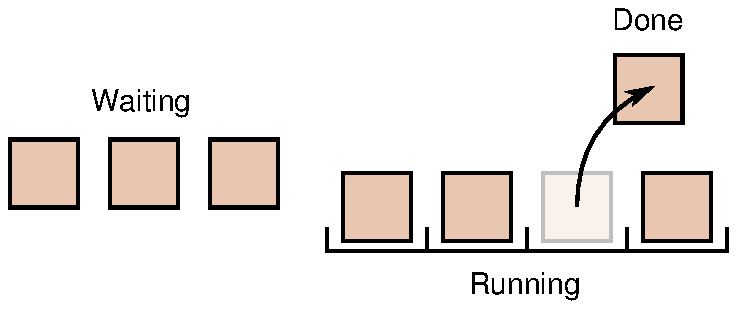
\includegraphics[width=0.75\linewidth]{blocks.pdf}
%% \end{center}
%% \end{frame}

%% \begin{frame}{What what's a kernel? What are (CUDA) threads?}
%% \vspace{0.5 cm}

%% \begin{center}
%% 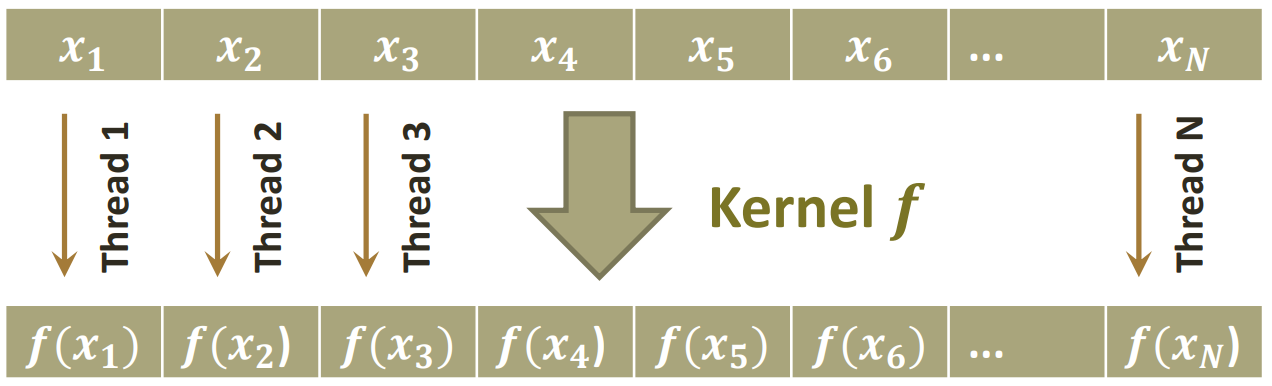
\includegraphics[width=0.85\linewidth]{threads.png}
%% \end{center}
%% \end{frame}

%% \begin{frame}[fragile]{Higher-level GPU programming: PyCUDA and Numba}
%% \vspace{0.25 cm}
%% \Large Install via Miniconda (Python 3). \textcolor{blue}{\normalsize\underline{\url{https://conda.io/miniconda.html}}}

%% \small
%% \begin{minted}{bash}
%% wget "https://repo.continuum.io/miniconda/"\
%% "Miniconda3-latest-Linux-x86_64.sh"
%% sh Miniconda3-latest-Linux-x86_64.sh      # ...and follow instructions

%% export PATH=/path/to/miniconda3/bin:$PATH
%% export LD_LIBRARY_PATH=/path/to/miniconda3/lib:$LD_LIBRARY_PATH
%% conda update conda

%% # PyCUDA
%% conda install -c lukepfister pycuda

%% # Numba with CUDA extensions
%% conda install cudatoolkit
%% conda install numba
%% \end{minted}
%% \end{frame}

%% \begin{frame}[fragile]{PyCUDA version of the program we compiled with nvcc}
%% \vspace{0.1 cm}
%% \scriptsize
%% \begin{minted}{python}
%% import numpy
%% import pycuda.autoinit
%% import pycuda.compiler
%% import pycuda.driver

%% module = pycuda.compiler.SourceModule("""
%% __global__ void gpu_kernel(float* datain, float* dataout) {
%%   int id = threadIdx.x + blockIdx.x*blockDim.x;
%%   dataout[id] = sqrt(datain[id]);
%% }
%% """)
%% gpu_kernel = module.get_function("gpu_kernel")

%% MILLION = 1024*1024
%% cpu_datain = numpy.random.uniform(0.0, 1.0, MILLION).astype(numpy.float32)
%% cpu_dataout = numpy.empty(MILLION, numpy.float32)

%% gpu_kernel(pycuda.driver.In(cpu_datain),
%%            pycuda.driver.Out(cpu_dataout),
%%            block=(1024, 1, 1),
%%            grid=(MILLION // 1024, 1))

%% print("first:", cpu_datain[0], "-->", cpu_dataout[0])
%% \end{minted}
%% \end{frame}

%% \begin{frame}[fragile]{Or PyCUDA with GPUArrays}
%% \vspace{0.2 cm}
%% \scriptsize
%% \begin{minted}{python}
%% import numpy
%% import pycuda.autoinit
%% import pycuda.elementwise
%% import pycuda.gpuarray

%% gpu_kernel = pycuda.elementwise.ElementwiseKernel(
%%     "float* datain, float* dataout",
%%     "dataout[i] = sqrt(datain[i])",
%%     "gpu_kernel")

%% MILLION = 1024*1024
%% cpu_datain = numpy.random.uniform(0.0, 1.0, MILLION).astype(numpy.float32)

%% gpu_datain = pycuda.gpuarray.to_gpu(cpu_datain)
%% gpu_dataout = pycuda.gpuarray.empty(MILLION, numpy.float32)
%% gpu_kernel(gpu_datain, gpu_dataout)

%% print("first:", cpu_datain[0], "-->", gpu_dataout[0])
%% \end{minted}

%% \vspace{0.15 cm}
%% \normalsize
%% or even

%% \vspace{0.15 cm}
%% \scriptsize
%% \begin{minted}{python}
%% import pycuda.cumath
%% gpu_dataout = pycuda.cumath.sqrt(gpu_datain)
%% \end{minted}
%% \end{frame}

\begin{frame}[fragile]{Numba version of the program we compiled with nvcc}
\vspace{0.1 cm}
\scriptsize
\begin{minted}{python}
import math
import numpy
import numba.cuda

@numba.cuda.jit
def gpu_kernel(datain, dataout):
    id = numba.cuda.grid(1)   # shortcut for threadIdx etc. with 1 dimension
    dataout[id] = math.sqrt(datain[id])

MILLION = 1024*1024
cpu_datain = numpy.random.uniform(0.0, 1.0, MILLION).astype(numpy.float32)

gpu_datain = numba.cuda.to_device(cpu_datain)
gpu_dataout = numba.cuda.device_array(MILLION, numpy.float32)
gpu_kernel[MILLION // 1024, 1024](gpu_datain, gpu_dataout)

print("first:", cpu_datain[0], "-->", gpu_dataout[0])
\end{minted}
\end{frame}


\end{document}
